% Template for ESA 6th ICATT manuscripts; to be used with:
%          spconf.sty  - LaTeX style file, and
%          IEEEbib.bst - IEEE bibliography style file.
% --------------------------------------------------------------------------
\documentclass{article}
\usepackage{spconf,amsmath,graphicx, url, listings}
\usepackage{courier, float}
\usepackage{caption}
\usepackage{subcaption}


\lstset{basicstyle=\footnotesize\ttfamily, float, language=MATLAB, breaklines=true}

% Example definitions.
% --------------------
\def\x{{\mathbf x}}
\def\L{{\cal L}}

% Title.
% ------
\title{Dynamic Optimisation of Tilt-A-Whirl}
%
% Single address.
% ---------------
\name{Christopher Iliffe Sprague}
\address{}
%
% For example:
% ------------
%\address{School\\
%	Department\\
%	Address}
%
% Two addresses (uncomment and modify for two-address case).
% ----------------------------------------------------------
%\twoauthors
%  {A. Author-one, B. Author-two\sthanks{Thanks to XYZ agency for funding.}}
%	{School A-B\\
%	Department A-B\\
%	Address A-B}
%  {C. Author-three, D. Author-four\sthanks{The fourth author performed the work
%	while at ...}}
%	{School C-D\\
%	Department C-D\\
%	Address C-D}
%
\begin{document}

\maketitle

\begin{abstract}
This paper examines the design optimization of a Tilt-A-Whirl ride, as an extension of Kautz's \textit{Chaos at the amusement park: Dynamics of the Tilt-A-Whirl} \cite{Kautz1994}. In particular, the task of optimizing passenger experience is analyzed and solved. The objective, the passenger's enjoyment, is approximated by the standard deviation of each car's intrinsic angular velocity, found through numerical integration. A Gaussian process surrogate model is used to approximate the system's time dependent objective, in order to save on computationally intensive evaluations of the \textit{true} objective function. A hybrid particle swarm algorithm is used to optimize the ride's design parameters in order to maximize the passenger's enjoyment. It is shown that a final objective value of over 200\% better than the nominal, yielded from the parameters presented in \cite{Kautz1994}, is achievable.
\end{abstract}
    
\keywords{Amusement Ride, Design Optimization, Particle Swarm, Gaussian Process}

\tableofcontents
\listoffigures
\lstlistoflistings

\section{Background}
Following the work of \cite{Kautz1994}, the dynamical model of a Tilta-A-Whirl is revisited. Like many other dynamical systems governed by deterministic equations, the Tilt-A-Whirl is found to exhibit chaotic behavior. In the dynamical model being examined, each of the Tilt-A-Whirl cars are free to pivot about the center of their own circular platform. The platforms move along a hilly circular track that tilts the platforms in all possible directions. While the translation and orientation of the platforms are completely predictable, each car whirls around in an independent and chaotic fashion. 

\subsection{Parameters} \label{sec:param}
\subsubsection{Constants}
For this paper's application, there are three design variables which are taken to be constant at the nominal values presented in \cite{Kautz1994}, namely: the beam length from the center of the ride to the center of each platform $r_1=4.3~m$, the radial incline offset of the platform $\alpha_0 = 0.036~rad$, and the parameter $Q_0 = \left(m/\rho\right)\sqrt{gr_2^3} = 20$, where $m$ is the mass of the car, $\rho$ is a damping coefficient to account for friction, and $g$ is the acceleration due to gravity.

\subsubsection{Design}
For the design optimization problem analyzed in this paper, three parameters are chosen to be manipulable, namely: the extrinsic angular velocity of the platform $\omega = \dot{\theta} \in [0.3142,0.8378] ~ rad/s$, the length of the radial arm from the center of each platform to the approximate center of gravity of the car $r_2 \in \left[0.1,1.5\right]~m$, and the maximum/minimum incline angle of the beam from the center of the ride to the platform $\alpha_1 \in \left[0,0.3\right] ~ rad$. The nominal values of the design variables are given as $\{\omega,r_2,\alpha_1\}_0 = \{6.5\times(2\pi/60) ~rad/s, 0.8~m, 0.058~rad\}$. Both the constant parameters and variable design parameters can be seen within a clearer context in Figure \ref{fig:tawplan}. In an object-orientated manner, a Tilt-A-Whirl car can be programmatically instantiated with these nominal parameters and bounds, as shown in Listing \ref{caropt}. The remaining parameters are discussed in latter sections.

\begin{lstlisting}[caption=Nominal Tilt-A-Whirl Car, label=caropt]
% Instantiate car with
% nominal values.
TW = Car(              ...
    4.3,               ... r1 m
    0.036,             ... alpha0 rad
    20,                ... Q0
    0.68,              ... omega rad/s
    0.8,               ... r2 m
    0.058,             ... alpha1 rad
    [3, 8].*(2*pi/60), ... omega bounds rad/s
    [0.1, 1.5],        ... r2 bounds m
    [0,0.3],           ... alpha1 bounds rad
    2000,              ... tau duration
    100,               ... # of samples
    0.05               ... noise level
);
\end{lstlisting}

\begin{figure}

\begin{subfigure}{0.49\textwidth}
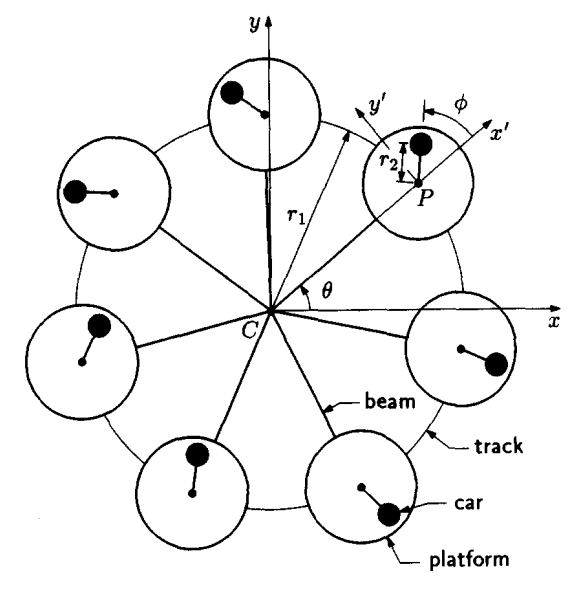
\includegraphics[width=0.9\linewidth]{Pics/tawplan.png} 
\caption{Overhead}
\end{subfigure}

\begin{subfigure}{0.49\textwidth}
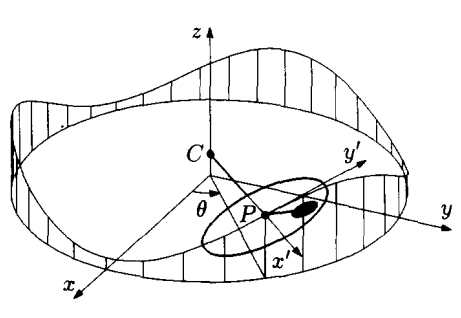
\includegraphics[width=0.9\linewidth]{Pics/tawperspective.png}
\caption{Three dimensional}
\end{subfigure}

\begin{subfigure}{0.49\textwidth}
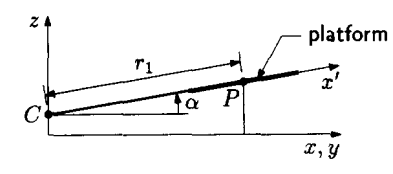
\includegraphics[width=0.9\linewidth]{Pics/tawtangential.png}
\caption{Tangential}
\end{subfigure}

\begin{subfigure}{0.49\textwidth}
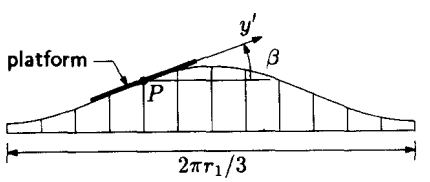
\includegraphics[width=0.9\linewidth]{Pics/tawradial.png}
\caption{Radial}
\end{subfigure}
 
\caption{Views of the Tilt-A-Whirl model.}
\cite{Kautz1994}
\label{fig:tawplan}
\end{figure}

\subsection{Equation of Motion}
From \cite{Kautz1994}, the second order differential equation of motion governing the Tilt-A-Whirl is defined as
\begin{equation}
\label{eq:motion}
\frac{d^2\phi}{d\tau^2} + \frac{\gamma}{Q_0} \frac{d\phi}{d\tau} + \left(\epsilon - \gamma^2\alpha \right) \sin\left(\phi\right) + \gamma^2\beta\cos\left(\phi\right) = 0
\end{equation}
, where the dimensionless parameters are defined as 
\begin{gather}
\tau = 3\omega t \\
\gamma = \frac{1}{3\omega} \sqrt{\frac{g}{r_2}}  \\
\epsilon = \frac{r_1}{9r_2} \\
\alpha = \alpha_0 - \alpha_1 \cos \left( \tau \right) \\
\beta = 3 \alpha_1 \sin \left(\tau\right)
\end{gather}
Programmatically, these equations of motion are transcribed as a first order system in Listing \ref{motion}.
\begin{lstlisting}[caption=Equations of Motion, label=motion]
function dphi = Rate(self, tau, phi)
    % Describes the Tilt-A-Whirl's
    % second order ordinary differential
    % equations of motion.
    p         = phi(1); % p
    dp        = phi(2); % p'
    dphi(1,1) = dp;     % p''
    % The system dynamics from
    % Eq. (27) of "Chaos at the amusement
    % park: Dynamics of the Tilt-A-Whirl
    % (Kautz and Huggard):
    g     = 9.802;
    gamma = 1/(3*self.omega);
    gamma = sqrt(g/self.r2)*gamma;
    eps   = self.r1/(9*self.r2);
    alpha = -self.alpha1*cos(tau);
    alpha = alpha+self.alpha0;
    beta  = 3*self.alpha1*sin(tau);
    d2p   = -(eps-(gamma^2)*alpha)*sin(p);
    d2p   = d2p-(gamma/self.Q0)*dp;
    d2p   = d2p-gamma^2*beta*cos(p);
    dphi(2,1) = d2p;
end
\end{lstlisting}

\subsection{Numerical Integration} \label{sec:int}
Of course, because Equation \ref{eq:motion} is rather nonlinear and chaotic, an analytical closed form solution does not exist. Thus, in order to observe the behavior of the system over time, it is necessary to numerically integrate the equation of motion. From a programmatic approach, one can implement Matlab's \textit{ode45} \cite{Matlab}, using the widely popular Runge-Kutta method of fourth and fifth order. From the object oriented appoach taken in this paper, this process manifests itself in the form of Listing \ref{ode}.
\begin{lstlisting}[caption=Numerical Integration, label=ode]
function [phi, t] = Propogate(self)
    % Propogates dynamics over over
    % dimensionless time.
    T        = self.T;
    [t, phi] = ode45(@self.Rate,[0,T],[0,0]);
end
\end{lstlisting}

\section{Optimization}
It is supposed that the unpredictability of each car's intrinsic angular velocity $\dot{\phi}$ is directly correlated to passenger enjoyment. Thus the objective measure of design performance is defined as the standard deviation of each car's intrinsic angular velocity $\sigma\left(\frac{d\phi}{dt}\right)$, where $\frac{d\phi}{dt}$ is obtained through numerical integration, as discussed in Section \ref{sec:int}.

\subsection{True Objective Function}
 Herein, the \textit{true} objective function $\sigma\left(\frac{d\phi}{dt}\right)$ is referred to as a function of design parameters $\sigma\left(\omega,r_2,\alpha_1\right)$, or less verbosely as $\sigma$. After numerical integration of the system's dynamics, a large list of $\dot{\phi}$ data points are obtained, from which the computation of $\sigma$ draws from. However, because the system's dynamics, described in Equation \ref{eq:motion}, are with respect to the non-dimensional parameter $\tau$, it is necessary to redimensionalize when computing the standard deviation of the car's intrinsic angular velocity. The programmatic transcription of this objective function is seen in Listing \ref{obj}.
 \begin{lstlisting}[caption=\textit{True} Objective Function, label=obj]
 function [stdp, phi, t] = StdPhi(self)
    % Returns standard deviations of dphi/dt.
    [phi,t] = self.Propogate();
    % Sample terminal dynamics only.
    el      = length(phi);  % End index
    tl      = round(el/3);  % Term index
    y       = phi(tl:el,2); % Term sample
    yb      = mean(y);
    stdp    = mean((y-yb).^2);
    stdp    = 3*self.omega*sqrt(stdp);
end
 \end{lstlisting}
Note that only the last two thirds of the $\dot{\phi}$ data points are taken into account. This is done to disregard the start-up of the system, and only take heed to the terminal dynamics, so as to compute a purer standard deviation.

The nature of the \textit{true} objective function $\sigma$ can be seen by keeping $\alpha_1$ and $r_2$ constant, while manipulating $\omega$, as shown in Figure \ref{fig:noise}. Of course, the evaluation of this objective function is quite computationally expensive, as each evaluation elicits the numerical integration of the system's equation of motion. It can also be seen that the \textit{true} objective function is rather noisy, not lending itself well to gradient based optimizers, such as \textit{fmincon} \cite{Matlab}, at all. A conventional optimization algorithm would indeed become trapped within the multiple local extrema that are exhibited.

\subsection{Problem Statement}
Taking note of the nominal constant parameter values and design parameter bounds described in Section \ref{sec:param}, the statement of the optimization problem is more formally formulated as
\begin{equation}
\begin{aligned}
& \underset{\omega, r_2, \alpha_1}{\text{minimize}} 
& & \sigma\left(\omega,r_2,\alpha_1\right) \\
& \text{subject to}
& & 3 \leq \omega\frac{60}{2\pi} \leq 8 ~ rpm \\
& & & 0.1 \leq r_2 \leq 1.5 ~m\\
& & & 0 \leq \alpha_1 \leq 0.3 ~ rad
\end{aligned}
\end{equation}

\begin{figure}
    \centering
    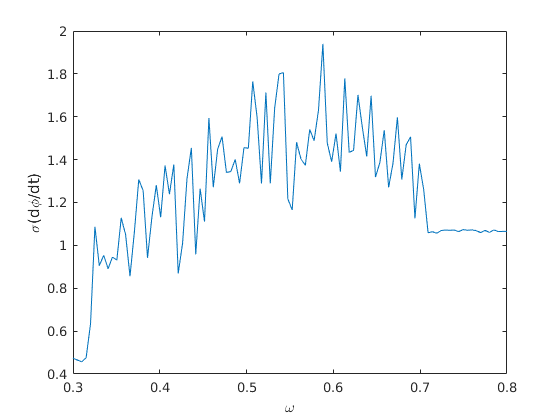
\includegraphics[width=0.48\textwidth]{Pics/stddphi.png}
    \caption{True Objective Function Sampling $\sigma(\omega)$}
    \label{fig:noise}
\end{figure}

\subsection{Surrogate model}
Because the \textit{true} objective function $\sigma$ is so noisy, chaotic, and computationally costly to evaluate, the appropriate course of action is to model the system's time-dependent behavior with a surrogate model.

\subsubsection{Sampling} \label{sec:lhs}
The \textit{true} objective function is sampled at various design parameter values using Latin hypercube sampling, with the use of \textit{lhsdesign} \cite{Matlab}. Latin hypercube sampling allows for near random sampling of the design space, to allow for the proper construction of the surrogate model. Programmatically this sampling is transcribed as shown in Listing \ref{lhssamp}.
\begin{lstlisting}[caption=Latin Hypercube Sampling, label=lhssamp]
function [stphi, x] = LHS_Sampling(self)
  % Define sample points with latin
  % hyper cube sampling.
  % # Variables
  n = length(self.Design_Vector());
  s = self.samps; % # of samples
  x = lhsdesign(s,n);
  % Variable bounds
  xl = [self.omegab(1);
        self.r2b(1);
        self.alpha1b(1)];
  xu = [self.omegab(2);
        self.r2b(2);
        self.alpha1b(2)];
  % Scaling according to bounds
  for i = 1:n
    x(:,i) = x(:,i).*(xu(i) - xl(i));
    x(:,i) = x(:,i) + xl(i);
  end
  % Evaluate objective function
  % at LHS samples
  ndes = length(x); % # designs
  for i = 1:ndes
    self.omega  = x(i,1);
    self.r2     = x(i,2);
    self.alpha1 = x(i,3);
    stphi(i,1)  = self.StdPhi();
  end
end
\end{lstlisting}
It is important to note that, initially, the sample values returned by \textit{lhsdesign} are not scaled to the problem's parameters; scaling must be done according the scale length of the problem's bounds. The function shown in Listing \ref{lhssamp} returns both the sample design parameter values and the \textit{true} objective function values at those parameters. The reader is encouraged to consult \cite{Helton2003} for a rigorous analysis of Latin hypercube sampling.

\subsubsection{Gaussian Process}
Using the work of Rasmussen \cite{Rasmussen2004}, a Gaussian process surrogate model is constructed to approximate the computationally expensive \textit{true} objective function. The Gaussian process library is a machine learning library that addresses the supervised learning problem of mapping inputs to outputs, with previous knowledge of labelled training data. Using the Latin hypercube sampling described in Section \ref{sec:lhs}, the surrogate model training process is instantiated in Listing \ref{gauss}, from which the Gaussian process hyperparameters are returned. 

Using the \textit{true} objective function samples, the surrogate model effectively learns the topology of the design space, through the training occurring during \lstinline{hyp = minimize(hyp, @gp, -100,@infExact,[],@covSEiso, @likGauss, xs, ys)}, in which the Gaussian process hyperparameters are minimized. Note that, in Listing \ref{gauss}, the hyperparameters and sampling points are saved, and used later unless the Gaussian process parameters have changed. This allows for significantly faster work-flow when testing different optimization algorithms.

\begin{lstlisting}[caption=Gaussian Process Hyperparameters, label=gauss]
function [hyp, xs, ys] = GP_Hyper(self)
  % Hyperparameters exist?
  if exist('Hyper.mat','file') == 2
    load('Hyper.mat');
    % Want a different sampling?
    if (self.samps ~= length(xs) ...
        || self.noise ~= ns      ...
        || self.T ~= T)
      disp('Different sampling...');
      need = true; % Then sample again
    else
      need = false; % Otherwise don't
    end
  else
    disp('Need sampling...');
    need = true; % No such file :(
  end
  if need == true
    % Latin hyper cube sampling
    [ys, xs]  = self.LHS_Sampling();
    % Set Matern covariance function
    covfunc   = {@covMaterniso, 1};
    % hyp.cov = [log(1); lfilefileog(sigma)];
    hyp.cov   = log([1/4;1.0]);
    % Gaussian likelihood function
    likfunc   = @likGauss;
    % Noise
    ns = self.noise;
    hyp.lik   = log(ns);
    % Minimise negative log
    % likelihood function
    disp('Minimising negative log likelihood function...');
    hyp = minimize(...
      hyp, @gp, -100, @infExact, ...
      [], @covSEiso, @likGauss, xs, ys ...
    );
    T = self.T;
    % Save for later
    save('Hyper','hyp','xs','ys','ns','T')
  end
end
\end{lstlisting}

From the Gaussian process hyperparameters returned from Listing \ref{gauss}, the surrogate model in Listing \ref{sur} acts as a callable function, herein refereed to as $\hat{\sigma}$, that can be \textit{inexpensively} evaluated in the optimization process. One major advantage of the surrogate objective function $\hat{\sigma}$ in Listing \ref{sur} over the \textit{true} objective function $\sigma$ in Listing \ref{obj}, is that it is smooth and is much nicer to optimize, especially with gradient based methods.

\begin{lstlisting}[caption=Surrogate Objective Function, label=sur]
function [fval,s2] = GP_Surrogate(self, x)
  [hyp, xs, ys] = self.GP_Hyper();
  % Evaluate mean at variables
  [fval, s2] = gp(                 ...
    hyp, @infExact, [], @covSEiso, ...
    @likGauss, xs, ys, x           ...
  );
end
\end{lstlisting}

With the Gaussian process surrogate model transcribed in Listing \ref{sur}, the single varriable design space topologies can be seen with 95\% confidence bounds in Figure \ref{fig:gauss}, with 200 Latin hypercube samples. Note the vastly smoother topology in Figure \ref{fig:gauss} compared that of Figure \ref{fig:noise}.

\begin{figure}

\begin{subfigure}{0.49\textwidth}
\includegraphics[width=0.9\linewidth]{Pics/stddphi-omega.eps} 
\caption{$\hat{\sigma}(\omega)$ with $r_2, \alpha_1$ nominal.}
\end{subfigure}

\begin{subfigure}{0.49\textwidth}
\includegraphics[width=0.9\linewidth]{Pics/stddphi-r2.eps}
\caption{$\hat{\sigma}(r_2)$ with $\omega, \alpha_1$ nominal.}
\end{subfigure}

\begin{subfigure}{0.49\textwidth}
\includegraphics[width=0.9\linewidth]{Pics/stddphi-alpha1.eps}
\caption{$\hat{\sigma}(\alpha_1)$ with $\omega, r_2$ nominal.}
\end{subfigure}

\caption{Single Variable $\hat{\sigma}$}
\label{fig:gauss}
\end{figure}

With the use of \lstinline{function [X,Y,F] = Surface(self, cvar, np)}, the topology of the design space within the neighborhood of the nominal parameters can be seen in Figure \ref{fig:nomtop}. It can be seen that both $\hat{\sigma}(r_2,\alpha_1)$ and $\hat{\sigma}(\omega,\alpha_1)$ are fairly nice look, while $\hat{\sigma}(\omega,r_2)$ seems rather treacherous.

\begin{figure}

\begin{subfigure}{0.49\textwidth}
\includegraphics[width=0.9\linewidth]{Pics/surf-a1-r2-nom.eps} 
\caption{$\hat{\sigma}(r_2,\alpha_1)$ with $\omega$ nominal.}
\end{subfigure}

\begin{subfigure}{0.49\textwidth}
\includegraphics[width=0.9\linewidth]{Pics/surf-w-a1-nom.eps}
\caption{$\hat{\sigma}(\omega,\alpha_1)$ with $r_2$ nominal.}
\end{subfigure}

\begin{subfigure}{0.49\textwidth}
\includegraphics[width=0.9\linewidth]{Pics/surf-w-r2-nom.eps}
\caption{$\hat{\sigma}(\omega,r_2)$ with $\alpha_1$ nominal.}
\end{subfigure}

\caption{Nominal Multivariate $\hat{\sigma}$ Topology}
\label{fig:nomtop}
\end{figure}

\subsection{Particle Swarm} \label{ps}
Particle swarm is a population-based stochastic optimization algorithm. It solves an optimization problem by a population of possible solutions, otherwise known as particles, and moving the particles around in the design search space, according to the particles' positions and velocities. Every particle's movement is influenced by its best known local solution. However, the particles are also directed toward the best known positions in the design search space among other particles. In effect, this influences the swarm of particles to congregate upon the best solution. This optimization technique was inspired by the social behavior of bird flocking and fish school. The reader is encouraged to consult \cite{Kennedy1995} for more information on this algorithm. 

In order to implement this, Matlab's \textit{particleswarm} \cite{Matlab} function is used to optimize the surrogate function. This optimization algorithm is made particularly effective when parallelized on multiple CPU cores and augmented with the terminal use of a gradient based optimizer, such as \textit{fmincon} \cite{Matlab}. Essentially the particle swarm optimization coarsely hones in on the global optimum, at which point a gradient based optimizer pinpoints the solution, assuming the design space is sufficiently convex within the vicinity of the solution. 

The particle swarm optimization process can be intuitively commenced with \lstinline{[x,fval] = TW.Optimize('particle-swarm')}. With a Gaussian process surrogate model constructed with 100 samples, an objective standard deviation value of $\hat{\sigma}_{100} = 5.37419$ is obtained, as shown with convergence history in Figure \ref{fig:psconv100}. With 600 \textit{true} objective samples, a better objective of $\hat{\sigma}=6.17409$ is obtained, as seen in Figure \ref{fig:psconv600}.

\begin{figure}
    \centering
    \includegraphics[width=0.49\textwidth]{Pics/psfval100.eps}
    \caption{Hybrid Particle Swarm Convergence of $\hat{\sigma}$ with $N_s=100$}
    \label{fig:psconv100}
\end{figure}

\begin{figure}
    \centering
    \includegraphics[width=0.49\textwidth]{Pics/psfval600.eps}
    \caption{Hybrid Particle Swarm Convergence of $\hat{\sigma}$ with $N_s=600$}
    \label{fig:psconv600}
\end{figure}

Objective values returned by the optimizer tend to get better as the resolution of the \textit{true} objective function sampling increases, that is the number of samples $N_s$. However, it has been found that returns tend to decline as the resolution becomes very large. This is because, as the resolution of the surrogate function becomes greater, it exposes more detail of the \textit{true} design space. Small details which may have been disregarded at lower sample values, become apparent, as shown in Figure \ref{fig:psosamp}, giving surrogate objective values of $N_s = \{ 10,100,200,400,600,1000,2000\} \mapsto \hat{\sigma} = \{ 3.5879,4.0953,5.2154,6.2128,6.5701,6.2818,5.5852 \}$. However, the accuracy of the surrogate model and particle swarm optimization have been verified, yielding objective values over 200\% better than the nominal, for almost all values of $N_s$. The Gaussian process surrogate model's optimal design space topology can be seen in Figure \ref{fig:topopt}.

\begin{figure}
    \centering
    \includegraphics[width=0.49\textwidth]{Pics/psons.eps}
    \caption{Sampling Resolution and Surrogate Objective Returns}
    \label{fig:psosamp}
\end{figure}

\section{Results}
Through the particle swarm optimization process outlined in Section \ref{ps}, with $N_s=600$, an objective surrogate function value of $\hat{\sigma} = 6.1741$ is obtained with design parameters $\{\omega^*,r_2^*,\alpha_1^*\} = \{0.7703,0.1000,0.2716\}$. Evaluating the \textit{true} objective function $\sigma$ at these design parameters yields $\sigma(\omega^*,r_2^*,\alpha_1^*) = 6.6079$, thereby further guaranteeing the accuracy of the Gaussian process surrogate model implemented, and demonstrating a colossal 312.99\% improvement over the nominal $\sigma_{nom} = 1.6$. Interestingly, the optimal design parameter $r_2^*$ tends to converge to its lower bound.

\begin{figure}

\begin{subfigure}{0.49\textwidth}
\includegraphics[width=0.9\linewidth]{Pics/surf-a1-r2.eps} 
\caption{$\hat{\sigma}(r_2,\alpha_1)$ with $\omega$ optimal.}
\end{subfigure}

\begin{subfigure}{0.49\textwidth}
\includegraphics[width=0.9\linewidth]{Pics/surf-w-a1.eps}
\caption{$\hat{\sigma}(\omega,\alpha_1)$ with $r_2$ optimal.}
\end{subfigure}

\begin{subfigure}{0.49\textwidth}
\includegraphics[width=0.9\linewidth]{Pics/surf-w-r2.eps}
\caption{$\hat{\sigma}(\omega,r_2)$ with $\alpha_1$ optimal.}
\end{subfigure}

\caption{Optimal Multivariate $\hat{\sigma}$ Topology}
\label{fig:topopt}
\end{figure}

\bibliographystyle{ieeetr}
\bibliography{refs.bib}

\onecolumn
\section{Source Code}
\lstinputlisting[caption=Example Car Optimization, basicstyle=\ttfamily]{Code/Optimization.m}
\lstinputlisting[caption=Car Class,basicstyle=\ttfamily]{Code/Car.m}

\end{document}